\documentclass[conference]{IEEEtran}
% ---------------------------------------------------------------------------------------------------------------
% Every number in this file comes from numbers.tex, generated by scripts/make_numbers.py from the repository's
% result files. Figures: scripts/make_figs.py (data) and figs/*.tex (TikZ).
% ---------------------------------------------------------------------------------------------------------------
\usepackage[T1]{fontenc}
\usepackage{amsmath,amssymb}
\usepackage{graphicx}
\usepackage{booktabs}
\usepackage{array}
\usepackage[table]{xcolor}
\usepackage{tikz}
\usetikzlibrary{arrows.meta,positioning,calc}
\usepackage{pifont}
\usepackage{algorithm}
\usepackage{algpseudocode}
\usepackage{cite}
\usepackage[hidelinks]{hyperref}
\usepackage{microtype}
% Generated by scripts/make_numbers.py -- do not edit by hand.
\newcommand{\NumCasCalibOneTwoEightS}{11}
\newcommand{\NumCasCalibSixteenS}{1.4}
\newcommand{\NumCasCalibThreeTwoS}{2.7}
\newcommand{\NumCasCwFactoryFprAll}{0.26}
\newcommand{\NumCasCwGFivenOneSixFpr}{0.023}
\newcommand{\NumCasCwGFivenOneSixTpr}{0.999}
\newcommand{\NumCasCwGFivenThreeTwoFpr}{0.037}
\newcommand{\NumCasCwGFivenThreeTwoTpr}{0.999}
\newcommand{\NumCasCwGFourFpr}{0.98}
\newcommand{\NumCasCwGFourTpr}{0.99}
\newcommand{\NumCasCwGOneFpr}{0.42}
\newcommand{\NumCasCwGOneTpr}{1.00}
\newcommand{\NumCasCwGThreeFpr}{1.00}
\newcommand{\NumCasCwGThreeTpr}{1.00}
\newcommand{\NumCasCwGTwoFpr}{1.00}
\newcommand{\NumCasCwGTwoTpr}{1.00}
\newcommand{\NumCasCwPayback}{8}
\newcommand{\NumCasCwSaving}{4.7}
\newcommand{\NumCasCwSelfFprAll}{0.075}
\newcommand{\NumCasEpiCwruGFive}{12.3}
\newcommand{\NumCasEpiCwruGOne}{31.3}
\newcommand{\NumCasEpiPuGOne}{100.5}
\newcommand{\NumCasEpiPuGSix}{54.2}
\newcommand{\NumCasPuModelE}{93}
\newcommand{\NumCasPuRuleE}{102}
\newcommand{\NumCasPuRuleNGates}{45}
\newcommand{\NumCasPuRuleNPass}{8}
\newcommand{\NumCasPuSaving}{1.7}
\newcommand{\NumCasPuSixNOneTwoEightE}{59}
\newcommand{\NumCasPuSixNOneTwoEightFprPFour}{0.016}
\newcommand{\NumCasPuSixNOneTwoEightFprPThree}{0.012}
\newcommand{\NumCasPuSixNOneTwoEightTprPFour}{1.00}
\newcommand{\NumCasPuSixNOneTwoEightTprPThree}{0.989}
\newcommand{\NumCasPuSixNSixFourE}{61}
\newcommand{\NumCasPuSixNSixFourFprPFour}{0.051}
\newcommand{\NumCasPuSixNSixFourFprPThree}{0.032}
\newcommand{\NumCasPuSixNSixFourTprPFour}{1.00}
\newcommand{\NumCasPuSixNSixFourTprPThree}{0.994}
\newcommand{\NumCwruAddMed}{0.13\,\%}
\newcommand{\NumCwruBestRankOnPu}{49}
\newcommand{\NumCwruBigCnnEstS}{20.9}
\newcommand{\NumCwruBigCnnId}{\texttt{cnn-r0-w200d4-fp32}}
\newcommand{\NumCwruBigCnnMeasS}{2.62}
\newcommand{\NumCwruCNNEMax}{64{,}757}
\newcommand{\NumCwruCNNEMed}{2{,}346}
\newcommand{\NumCwruCNNEMin}{607}
\newcommand{\NumCwruCNNFlashMaxKB}{324}
\newcommand{\NumCwruCNNFlashMinKB}{4.0}
\newcommand{\NumCwruCNNFrontShare}{0.2\,\%}
\newcommand{\NumCwruCNNN}{24}
\newcommand{\NumCwruCNNRunMax}{64{,}921}
\newcommand{\NumCwruCNNRunMin}{600}
\newcommand{\NumCwruCNNTMaxMs}{2{,}619}
\newcommand{\NumCwruCNNTMinMs}{28}
\newcommand{\NumCwruCalibGFiveNOneSix}{352}
\newcommand{\NumCwruCalibGFiveNThreeTwo}{624}
\newcommand{\NumCwruCasAgree}{1{,}046}
\newcommand{\NumCwruCasChecks}{1{,}046}
\newcommand{\NumCwruCasRepCv}{0.44\,\%}
\newcommand{\NumCwruCnnEMaxMJ}{65}
\newcommand{\NumCwruCnnEMinMJ}{0.61}
\newcommand{\NumCwruCnnOverTreeMax}{4{,}729}
\newcommand{\NumCwruCnnOverTreeMin}{44}
\newcommand{\NumCwruCvMax}{0.91\,\%}
\newcommand{\NumCwruCvMed}{0.17\,\%}
\newcommand{\NumCwruDTEMax}{88.8}
\newcommand{\NumCwruDTEMed}{56.7}
\newcommand{\NumCwruDTEMin}{13.7}
\newcommand{\NumCwruDTFlashMaxKB}{2.1}
\newcommand{\NumCwruDTFlashMinKB}{0.24}
\newcommand{\NumCwruDTFrontShare}{99.8\,\%}
\newcommand{\NumCwruDTN}{12}
\newcommand{\NumCwruDTRunMax}{0.11}
\newcommand{\NumCwruDTRunMin}{0.089}
\newcommand{\NumCwruDTTMaxMs}{3.9}
\newcommand{\NumCwruDTTMinMs}{0.64}
\newcommand{\NumCwruDropAll}{0.407}
\newcommand{\NumCwruDropCNN}{0.424}
\newcommand{\NumCwruDropDT}{0.281}
\newcommand{\NumCwruDropMLP}{0.401}
\newcommand{\NumCwruDropRF}{0.398}
\newcommand{\NumCwruEstRatioMax}{5.35}
\newcommand{\NumCwruEstRatioMed}{2.83}
\newcommand{\NumCwruEstRatioMin}{0.31}
\newcommand{\NumCwruEstRatioNnMax}{5.35}
\newcommand{\NumCwruEstRatioNnMin}{0.31}
\newcommand{\NumCwruEstRatioTreeMax}{3.15}
\newcommand{\NumCwruEstRatioTreeMin}{2.53}
\newcommand{\NumCwruEstSpearman}{0.997}
\newcommand{\NumCwruFlashMaxKB}{324}
\newcommand{\NumCwruFlashMinKB}{0.2}
\newcommand{\NumCwruFrontKept}{2}
\newcommand{\NumCwruFrontPOneN}{9}
\newcommand{\NumCwruFrontRFour}{86.4}
\newcommand{\NumCwruFrontROne}{13.6}
\newcommand{\NumCwruFrontRThree}{157}
\newcommand{\NumCwruFrontRTwo}{55.9}
\newcommand{\NumCwruFrontRZero}{4.81}
\newcommand{\NumCwruFrontTRFour}{3.90}
\newcommand{\NumCwruFrontTROne}{0.64}
\newcommand{\NumCwruFrontTRThree}{7.26}
\newcommand{\NumCwruFrontTRTwo}{2.50}
\newcommand{\NumCwruFrontTRZero}{0.17}
\newcommand{\NumCwruGateCvMax}{0.4\,\%}
\newcommand{\NumCwruGateEGFive}{9.7}
\newcommand{\NumCwruGateEGFour}{9.8}
\newcommand{\NumCwruGateEGOne}{7.7}
\newcommand{\NumCwruGateEGThree}{9.8}
\newcommand{\NumCwruGateEGTwo}{9.8}
\newcommand{\NumCwruGateEMax}{9.8}
\newcommand{\NumCwruGateEMin}{7.7}
\newcommand{\NumCwruGateRatioMax}{2.6}
\newcommand{\NumCwruGateRatioMin}{2.2}
\newcommand{\NumCwruIdleHi}{18.88}
\newcommand{\NumCwruIdleJh}{68}
\newcommand{\NumCwruIdleLo}{18.55}
\newcommand{\NumCwruIdleMed}{18.78}
\newcommand{\NumCwruIdleSpreadMW}{0.33}
\newcommand{\NumCwruIncJhOneS}{0.066}
\newcommand{\NumCwruLatRatioMax}{2.48}
\newcommand{\NumCwruLatRatioMed}{1.27}
\newcommand{\NumCwruLatRatioMin}{0.13}
\newcommand{\NumCwruLfEtoeSaveMax}{59\,\%}
\newcommand{\NumCwruLfFactorRFour}{1.21}
\newcommand{\NumCwruLfFactorROne}{1.13}
\newcommand{\NumCwruLfFactorRThree}{3.17}
\newcommand{\NumCwruLfFactorRTwo}{1.12}
\newcommand{\NumCwruLfFactorRZero}{1.00}
\newcommand{\NumCwruLfFrontRFour}{71.6}
\newcommand{\NumCwruLfFrontROne}{12.0}
\newcommand{\NumCwruLfFrontRThree}{49.3}
\newcommand{\NumCwruLfFrontRTwo}{49.4}
\newcommand{\NumCwruLfFrontRZero}{4.13}
\newcommand{\NumCwruLfImageShift}{11}
\newcommand{\NumCwruLfModels}{51}
\newcommand{\NumCwruLfReps}{3}
\newcommand{\NumCwruLfSaveRFour}{17\,\%}
\newcommand{\NumCwruLfSaveROne}{11\,\%}
\newcommand{\NumCwruLfSaveRThree}{68\,\%}
\newcommand{\NumCwruLfSaveRTwo}{11\,\%}
\newcommand{\NumCwruLfSaveRZero}{0\,\%}
\newcommand{\NumCwruMLPEMax}{307}
\newcommand{\NumCwruMLPEMed}{94.2}
\newcommand{\NumCwruMLPEMin}{59.4}
\newcommand{\NumCwruMLPFlashMaxKB}{135}
\newcommand{\NumCwruMLPFlashMinKB}{3.2}
\newcommand{\NumCwruMLPFrontShare}{82.3\,\%}
\newcommand{\NumCwruMLPN}{26}
\newcommand{\NumCwruMLPRunMax}{146}
\newcommand{\NumCwruMLPRunMin}{5.2}
\newcommand{\NumCwruMLPTMaxMs}{14}
\newcommand{\NumCwruMLPTMinMs}{2.7}
\newcommand{\NumCwruNModels}{80}
\newcommand{\NumCwruPOneBest}{1.000}
\newcommand{\NumCwruPOneBestCNN}{1.000}
\newcommand{\NumCwruPOneBestDT}{0.989}
\newcommand{\NumCwruPOneBestE}{5{,}856}
\newcommand{\NumCwruPOneBestId}{\texttt{cnn-r0-w050d4-fp32}}
\newcommand{\NumCwruPOneBestMLP}{1.000}
\newcommand{\NumCwruPOneBestRF}{0.997}
\newcommand{\NumCwruPOneEstFrontDiff}{4}
\newcommand{\NumCwruPOneEstFrontN}{9}
\newcommand{\NumCwruPOneHvAll}{1.246}
\newcommand{\NumCwruPOneHvCNN}{0.505}
\newcommand{\NumCwruPOneHvDT}{1.224}
\newcommand{\NumCwruPOneHvExclCNN}{0.000}
\newcommand{\NumCwruPOneHvExclDT}{0.332}
\newcommand{\NumCwruPOneHvExclMLP}{0.004}
\newcommand{\NumCwruPOneHvExclRF}{0.000}
\newcommand{\NumCwruPOneHvMLP}{0.755}
\newcommand{\NumCwruPOneHvRF}{0.900}
\newcommand{\NumCwruPOneNFront}{9}
\newcommand{\NumCwruPOneNFrontCNN}{0}
\newcommand{\NumCwruPOneNFrontDT}{3}
\newcommand{\NumCwruPOneNFrontMLP}{3}
\newcommand{\NumCwruPOneNFrontRF}{3}
\newcommand{\NumCwruPOneNFrontThree}{16}
\newcommand{\NumCwruPOneNearE}{57.1}
\newcommand{\NumCwruPOneNearFOne}{0.995}
\newcommand{\NumCwruPOneNearId}{\texttt{rf-r2-t5d10-fp32}}
\newcommand{\NumCwruPOneNearSaving}{103}
\newcommand{\NumCwruPThreeBest}{0.742}
\newcommand{\NumCwruPThreeBestCNN}{0.594}
\newcommand{\NumCwruPThreeBestDT}{0.719}
\newcommand{\NumCwruPThreeBestE}{90.1}
\newcommand{\NumCwruPThreeBestId}{\texttt{rf-r4-t25d6-fp32}}
\newcommand{\NumCwruPThreeBestMLP}{0.653}
\newcommand{\NumCwruPThreeBestRF}{0.742}
\newcommand{\NumCwruPThreeEstFrontDiff}{3}
\newcommand{\NumCwruPThreeEstFrontN}{6}
\newcommand{\NumCwruPThreeHvAll}{1.155}
\newcommand{\NumCwruPThreeHvCNN}{0.276}
\newcommand{\NumCwruPThreeHvDT}{1.118}
\newcommand{\NumCwruPThreeHvExclCNN}{0.000}
\newcommand{\NumCwruPThreeHvExclDT}{0.374}
\newcommand{\NumCwruPThreeHvExclMLP}{0.000}
\newcommand{\NumCwruPThreeHvExclRF}{0.035}
\newcommand{\NumCwruPThreeHvMLP}{0.553}
\newcommand{\NumCwruPThreeHvRF}{0.780}
\newcommand{\NumCwruPThreeNFront}{9}
\newcommand{\NumCwruPThreeNFrontCNN}{0}
\newcommand{\NumCwruPThreeNFrontDT}{6}
\newcommand{\NumCwruPThreeNFrontMLP}{0}
\newcommand{\NumCwruPThreeNFrontRF}{3}
\newcommand{\NumCwruPThreeNFrontThree}{14}
\newcommand{\NumCwruPThreeNearE}{90.1}
\newcommand{\NumCwruPThreeNearFOne}{0.742}
\newcommand{\NumCwruPThreeNearId}{\texttt{rf-r4-t25d6-fp32}}
\newcommand{\NumCwruPThreeNearSaving}{1}
\newcommand{\NumCwruPTwoBest}{0.962}
\newcommand{\NumCwruPTwoBestCNN}{0.955}
\newcommand{\NumCwruPTwoBestDT}{0.913}
\newcommand{\NumCwruPTwoBestE}{58.0}
\newcommand{\NumCwruPTwoBestId}{\texttt{rf-r2-t25d10-fp32}}
\newcommand{\NumCwruPTwoBestMLP}{0.949}
\newcommand{\NumCwruPTwoBestRF}{0.962}
\newcommand{\NumCwruPTwoEstFrontDiff}{1}
\newcommand{\NumCwruPTwoEstFrontN}{7}
\newcommand{\NumCwruPTwoHvAll}{1.158}
\newcommand{\NumCwruPTwoHvCNN}{0.468}
\newcommand{\NumCwruPTwoHvDT}{1.081}
\newcommand{\NumCwruPTwoHvExclCNN}{0.001}
\newcommand{\NumCwruPTwoHvExclDT}{0.275}
\newcommand{\NumCwruPTwoHvExclMLP}{0.001}
\newcommand{\NumCwruPTwoHvExclRF}{0.025}
\newcommand{\NumCwruPTwoHvMLP}{0.703}
\newcommand{\NumCwruPTwoHvRF}{0.872}
\newcommand{\NumCwruPTwoNFront}{6}
\newcommand{\NumCwruPTwoNFrontCNN}{0}
\newcommand{\NumCwruPTwoNFrontDT}{1}
\newcommand{\NumCwruPTwoNFrontMLP}{0}
\newcommand{\NumCwruPTwoNFrontRF}{5}
\newcommand{\NumCwruPTwoNFrontThree}{20}
\newcommand{\NumCwruPTwoNearE}{58.0}
\newcommand{\NumCwruPTwoNearFOne}{0.962}
\newcommand{\NumCwruPTwoNearId}{\texttt{rf-r2-t25d10-fp32}}
\newcommand{\NumCwruPTwoNearSaving}{1}
\newcommand{\NumCwruPatchRatioMax}{1.014}
\newcommand{\NumCwruPatchRatioMed}{0.996}
\newcommand{\NumCwruPatchRatioMin}{0.972}
\newcommand{\NumCwruRFEMax}{90.4}
\newcommand{\NumCwruRFEMed}{57.3}
\newcommand{\NumCwruRFEMin}{14.3}
\newcommand{\NumCwruRFFlashMaxKB}{48}
\newcommand{\NumCwruRFFlashMinKB}{2.4}
\newcommand{\NumCwruRFFrontShare}{98.3\,\%}
\newcommand{\NumCwruRFN}{18}
\newcommand{\NumCwruRFRunMax}{1.3}
\newcommand{\NumCwruRFRunMin}{0.21}
\newcommand{\NumCwruRFTMaxMs}{4.0}
\newcommand{\NumCwruRFTMinMs}{0.65}
\newcommand{\NumCwruRankPLast}{DT>RF>MLP>CNN}
\newcommand{\NumCwruRankPOne}{DT>RF>MLP>CNN}
\newcommand{\NumCwruRejPct}{0.08\,\%}
\newcommand{\NumCwruRejected}{6}
\newcommand{\NumCwruRqEightFit}{18.3}
\newcommand{\NumCwruRqEightHi}{26.4}
\newcommand{\NumCwruRqEightLo}{10.1}
\newcommand{\NumCwruRqEightModel}{10.8}
\newcommand{\NumCwruRqFourFail}{4}
\newcommand{\NumCwruRqFourInMax}{2.6\,\%}
\newcommand{\NumCwruRqFourInMin}{0.6\,\%}
\newcommand{\NumCwruRqFourN}{15}
\newcommand{\NumCwruRqSixMax}{12.1}
\newcommand{\NumCwruRqSixMin}{11.9}
\newcommand{\NumCwruRqThreeFail}{6}
\newcommand{\NumCwruRqThreeInMax}{0.7\,\%}
\newcommand{\NumCwruRqThreeInMin}{0.5\,\%}
\newcommand{\NumCwruRqThreeMin}{$-$8.0\,\%}
\newcommand{\NumCwruRqThreeN}{8}
\newcommand{\NumCwruSessions}{29}
\newcommand{\NumCwruTauPOnePThree}{$-$0.21}
\newcommand{\NumCwruTauPOnePTwo}{0.42}
\newcommand{\NumCwruTauPTwoPThree}{0.00}
\newcommand{\NumCwruVerIntAgreeMin}{86\,\%}
\newcommand{\NumCwruVerIntFail}{29}
\newcommand{\NumCwruVerIntN}{29}
\newcommand{\NumCwruVerN}{80}
\newcommand{\NumCwruVerPass}{51}
\newcommand{\NumCwruVerTwoN}{50}
\newcommand{\NumCwruVerTwoPass}{50}
\newcommand{\NumCwruWindows}{7{,}527}
\newcommand{\NumHostAblMeanWith}{0.339}
\newcommand{\NumHostAblMeanWithout}{0.899}
\newcommand{\NumHostCmsisMax}{31.4}
\newcommand{\NumHostCmsisMedian}{17.6}
\newcommand{\NumHostCmsisMin}{5.9}
\newcommand{\NumHostMeanZMax}{16.6}
\newcommand{\NumHostPOneLeakPct}{98.1\,\%}
\newcommand{\NumNModelsBoth}{80}
\newcommand{\NumPuAddMed}{0.06\,\%}
\newcommand{\NumPuBigCnnEstS}{20.9}
\newcommand{\NumPuBigCnnId}{\texttt{cnn-r0-w200d4-fp32}}
\newcommand{\NumPuBigCnnMeasS}{2.60}
\newcommand{\NumPuCNNEMax}{65{,}457}
\newcommand{\NumPuCNNEMed}{2{,}374}
\newcommand{\NumPuCNNEMin}{607}
\newcommand{\NumPuCNNFlashMaxKB}{320}
\newcommand{\NumPuCNNFlashMinKB}{3.8}
\newcommand{\NumPuCNNFrontShare}{0.2\,\%}
\newcommand{\NumPuCNNN}{24}
\newcommand{\NumPuCNNRunMax}{65{,}563}
\newcommand{\NumPuCNNRunMin}{602}
\newcommand{\NumPuCNNTMaxMs}{2{,}599}
\newcommand{\NumPuCNNTMinMs}{28}
\newcommand{\NumPuCalibGFiveNOneSix}{371}
\newcommand{\NumPuCalibGFiveNThreeTwo}{653}
\newcommand{\NumPuCalibGSixNOneTwoEight}{12{,}644}
\newcommand{\NumPuCasAgree}{1{,}342}
\newcommand{\NumPuCasChecks}{1{,}342}
\newcommand{\NumPuCasRepCv}{0.38\,\%}
\newcommand{\NumPuCnnEMaxMJ}{65}
\newcommand{\NumPuCnnEMinMJ}{0.61}
\newcommand{\NumPuCnnOverTreeMax}{5{,}260}
\newcommand{\NumPuCnnOverTreeMin}{49}
\newcommand{\NumPuCvMax}{0.45\,\%}
\newcommand{\NumPuCvMed}{0.14\,\%}
\newcommand{\NumPuDTEMax}{88.9}
\newcommand{\NumPuDTEMed}{56.7}
\newcommand{\NumPuDTEMin}{13.6}
\newcommand{\NumPuDTFlashMaxKB}{13}
\newcommand{\NumPuDTFlashMinKB}{0.33}
\newcommand{\NumPuDTFrontShare}{99.9\,\%}
\newcommand{\NumPuDTN}{12}
\newcommand{\NumPuDTRunMax}{0.079}
\newcommand{\NumPuDTRunMin}{0.040}
\newcommand{\NumPuDTTMaxMs}{4.0}
\newcommand{\NumPuDTTMinMs}{0.64}
\newcommand{\NumPuDropAll}{0.321}
\newcommand{\NumPuDropCNN}{0.422}
\newcommand{\NumPuDropDT}{0.299}
\newcommand{\NumPuDropMLP}{0.319}
\newcommand{\NumPuDropRF}{0.287}
\newcommand{\NumPuEstRatioMax}{5.34}
\newcommand{\NumPuEstRatioMed}{2.70}
\newcommand{\NumPuEstRatioMin}{0.31}
\newcommand{\NumPuEstRatioNnMax}{5.34}
\newcommand{\NumPuEstRatioNnMin}{0.31}
\newcommand{\NumPuEstRatioTreeMax}{3.13}
\newcommand{\NumPuEstRatioTreeMin}{2.28}
\newcommand{\NumPuEstSpearman}{0.991}
\newcommand{\NumPuFlashMaxKB}{320}
\newcommand{\NumPuFlashMinKB}{0.3}
\newcommand{\NumPuFrontKept}{6}
\newcommand{\NumPuFrontPOneN}{15}
\newcommand{\NumPuFrontRFour}{85.2}
\newcommand{\NumPuFrontROne}{13.5}
\newcommand{\NumPuFrontRThree}{157}
\newcommand{\NumPuFrontRTwo}{55.3}
\newcommand{\NumPuFrontRZero}{5.27}
\newcommand{\NumPuFrontTRFour}{3.87}
\newcommand{\NumPuFrontTROne}{0.64}
\newcommand{\NumPuFrontTRThree}{7.24}
\newcommand{\NumPuFrontTRTwo}{2.50}
\newcommand{\NumPuFrontTRZero}{0.18}
\newcommand{\NumPuGateCvMax}{0.6\,\%}
\newcommand{\NumPuGateEGFive}{10.4}
\newcommand{\NumPuGateEGFour}{10.3}
\newcommand{\NumPuGateEGOne}{8.1}
\newcommand{\NumPuGateEGSix}{53.3}
\newcommand{\NumPuGateEGThree}{10.3}
\newcommand{\NumPuGateEGTwo}{10.4}
\newcommand{\NumPuGateEMax}{10.4}
\newcommand{\NumPuGateEMin}{8.1}
\newcommand{\NumPuGateRatioMax}{2.8}
\newcommand{\NumPuGateRatioMin}{2.3}
\newcommand{\NumPuIdleHi}{18.89}
\newcommand{\NumPuIdleJh}{68}
\newcommand{\NumPuIdleLo}{18.56}
\newcommand{\NumPuIdleMed}{18.78}
\newcommand{\NumPuIdleSpreadMW}{0.34}
\newcommand{\NumPuIncJhOneS}{0.244}
\newcommand{\NumPuLatRatioMax}{2.47}
\newcommand{\NumPuLatRatioMed}{1.23}
\newcommand{\NumPuLatRatioMin}{0.12}
\newcommand{\NumPuLfEtoeSaveMax}{59\,\%}
\newcommand{\NumPuLfFactorRFour}{1.20}
\newcommand{\NumPuLfFactorROne}{0.87}
\newcommand{\NumPuLfFactorRThree}{3.14}
\newcommand{\NumPuLfFactorRTwo}{1.09}
\newcommand{\NumPuLfFactorRZero}{0.99}
\newcommand{\NumPuLfFrontRFour}{71.5}
\newcommand{\NumPuLfFrontROne}{13.8}
\newcommand{\NumPuLfFrontRThree}{50.4}
\newcommand{\NumPuLfFrontRTwo}{49.9}
\newcommand{\NumPuLfFrontRZero}{4.14}
\newcommand{\NumPuLfImageShift}{15}
\newcommand{\NumPuLfModels}{52}
\newcommand{\NumPuLfReps}{3}
\newcommand{\NumPuLfSaveRFour}{17\,\%}
\newcommand{\NumPuLfSaveROne}{$-$15\,\%}
\newcommand{\NumPuLfSaveRThree}{68\,\%}
\newcommand{\NumPuLfSaveRTwo}{8\,\%}
\newcommand{\NumPuLfSaveRZero}{$-$1\,\%}
\newcommand{\NumPuMLPEMax}{304}
\newcommand{\NumPuMLPEMed}{91.9}
\newcommand{\NumPuMLPEMin}{57.7}
\newcommand{\NumPuMLPFlashMaxKB}{132}
\newcommand{\NumPuMLPFlashMinKB}{2.9}
\newcommand{\NumPuMLPFrontShare}{86.2\,\%}
\newcommand{\NumPuMLPN}{26}
\newcommand{\NumPuMLPRunMax}{145}
\newcommand{\NumPuMLPRunMin}{3.6}
\newcommand{\NumPuMLPTMaxMs}{13}
\newcommand{\NumPuMLPTMinMs}{2.6}
\newcommand{\NumPuNModels}{80}
\newcommand{\NumPuPFourBest}{0.479}
\newcommand{\NumPuPFourBestCNN}{0.439}
\newcommand{\NumPuPFourBestDT}{0.460}
\newcommand{\NumPuPFourBestE}{304}
\newcommand{\NumPuPFourBestId}{\texttt{mlp-r3-h128-fp32}}
\newcommand{\NumPuPFourBestMLP}{0.479}
\newcommand{\NumPuPFourBestRF}{0.432}
\newcommand{\NumPuPFourEstFrontDiff}{1}
\newcommand{\NumPuPFourEstFrontN}{4}
\newcommand{\NumPuPFourHvAll}{1.203}
\newcommand{\NumPuPFourHvCNN}{0.382}
\newcommand{\NumPuPFourHvDT}{1.141}
\newcommand{\NumPuPFourHvExclCNN}{0.000}
\newcommand{\NumPuPFourHvExclDT}{0.469}
\newcommand{\NumPuPFourHvExclMLP}{0.061}
\newcommand{\NumPuPFourHvExclRF}{0.002}
\newcommand{\NumPuPFourHvMLP}{0.672}
\newcommand{\NumPuPFourHvRF}{0.514}
\newcommand{\NumPuPFourNFront}{5}
\newcommand{\NumPuPFourNFrontCNN}{0}
\newcommand{\NumPuPFourNFrontDT}{1}
\newcommand{\NumPuPFourNFrontMLP}{3}
\newcommand{\NumPuPFourNFrontRF}{1}
\newcommand{\NumPuPFourNFrontThree}{5}
\newcommand{\NumPuPFourNearE}{178}
\newcommand{\NumPuPFourNearFOne}{0.472}
\newcommand{\NumPuPFourNearId}{\texttt{mlp-r3-h32-int8}}
\newcommand{\NumPuPFourNearSaving}{2}
\newcommand{\NumPuPOneBest}{0.967}
\newcommand{\NumPuPOneBestCNN}{0.965}
\newcommand{\NumPuPOneBestDT}{0.921}
\newcommand{\NumPuPOneBestE}{84.4}
\newcommand{\NumPuPOneBestId}{\texttt{mlp-r2-h64x64-fp32}}
\newcommand{\NumPuPOneBestMLP}{0.967}
\newcommand{\NumPuPOneBestRF}{0.939}
\newcommand{\NumPuPOneEstFrontDiff}{3}
\newcommand{\NumPuPOneEstFrontN}{16}
\newcommand{\NumPuPOneHvAll}{1.085}
\newcommand{\NumPuPOneHvCNN}{0.470}
\newcommand{\NumPuPOneHvDT}{0.984}
\newcommand{\NumPuPOneHvExclCNN}{0.000}
\newcommand{\NumPuPOneHvExclDT}{0.207}
\newcommand{\NumPuPOneHvExclMLP}{0.062}
\newcommand{\NumPuPOneHvExclRF}{0.010}
\newcommand{\NumPuPOneHvMLP}{0.790}
\newcommand{\NumPuPOneHvRF}{0.738}
\newcommand{\NumPuPOneNFront}{15}
\newcommand{\NumPuPOneNFrontCNN}{0}
\newcommand{\NumPuPOneNFrontDT}{1}
\newcommand{\NumPuPOneNFrontMLP}{9}
\newcommand{\NumPuPOneNFrontRF}{5}
\newcommand{\NumPuPOneNFrontThree}{24}
\newcommand{\NumPuPOneNearE}{61.3}
\newcommand{\NumPuPOneNearFOne}{0.961}
\newcommand{\NumPuPOneNearId}{\texttt{mlp-r2-h64-int8}}
\newcommand{\NumPuPOneNearSaving}{1}
\newcommand{\NumPuPThreeBest}{0.599}
\newcommand{\NumPuPThreeBestCNN}{0.520}
\newcommand{\NumPuPThreeBestDT}{0.519}
\newcommand{\NumPuPThreeBestE}{93.3}
\newcommand{\NumPuPThreeBestId}{\texttt{mlp-r4-h32-fp32}}
\newcommand{\NumPuPThreeBestMLP}{0.599}
\newcommand{\NumPuPThreeBestRF}{0.573}
\newcommand{\NumPuPThreeEstFrontDiff}{9}
\newcommand{\NumPuPThreeEstFrontN}{14}
\newcommand{\NumPuPThreeHvAll}{1.029}
\newcommand{\NumPuPThreeHvCNN}{0.310}
\newcommand{\NumPuPThreeHvDT}{0.684}
\newcommand{\NumPuPThreeHvExclCNN}{0.000}
\newcommand{\NumPuPThreeHvExclDT}{0.172}
\newcommand{\NumPuPThreeHvExclMLP}{0.117}
\newcommand{\NumPuPThreeHvExclRF}{0.037}
\newcommand{\NumPuPThreeHvMLP}{0.776}
\newcommand{\NumPuPThreeHvRF}{0.713}
\newcommand{\NumPuPThreeNFront}{13}
\newcommand{\NumPuPThreeNFrontCNN}{0}
\newcommand{\NumPuPThreeNFrontDT}{1}
\newcommand{\NumPuPThreeNFrontMLP}{4}
\newcommand{\NumPuPThreeNFrontRF}{8}
\newcommand{\NumPuPThreeNFrontThree}{26}
\newcommand{\NumPuPThreeNearE}{88.9}
\newcommand{\NumPuPThreeNearFOne}{0.591}
\newcommand{\NumPuPThreeNearId}{\texttt{mlp-r4-h16-int8}}
\newcommand{\NumPuPThreeNearSaving}{1}
\newcommand{\NumPuPTwoBest}{0.822}
\newcommand{\NumPuPTwoBestCNN}{0.813}
\newcommand{\NumPuPTwoBestDT}{0.745}
\newcommand{\NumPuPTwoBestE}{61.0}
\newcommand{\NumPuPTwoBestId}{\texttt{mlp-r2-h32-fp32}}
\newcommand{\NumPuPTwoBestMLP}{0.822}
\newcommand{\NumPuPTwoBestRF}{0.781}
\newcommand{\NumPuPTwoEstFrontDiff}{6}
\newcommand{\NumPuPTwoEstFrontN}{10}
\newcommand{\NumPuPTwoHvAll}{1.108}
\newcommand{\NumPuPTwoHvCNN}{0.461}
\newcommand{\NumPuPTwoHvDT}{0.919}
\newcommand{\NumPuPTwoHvExclCNN}{0.000}
\newcommand{\NumPuPTwoHvExclDT}{0.230}
\newcommand{\NumPuPTwoHvExclMLP}{0.100}
\newcommand{\NumPuPTwoHvExclRF}{0.004}
\newcommand{\NumPuPTwoHvMLP}{0.794}
\newcommand{\NumPuPTwoHvRF}{0.710}
\newcommand{\NumPuPTwoNFront}{10}
\newcommand{\NumPuPTwoNFrontCNN}{0}
\newcommand{\NumPuPTwoNFrontDT}{1}
\newcommand{\NumPuPTwoNFrontMLP}{4}
\newcommand{\NumPuPTwoNFrontRF}{5}
\newcommand{\NumPuPTwoNFrontThree}{18}
\newcommand{\NumPuPTwoNearE}{59.0}
\newcommand{\NumPuPTwoNearFOne}{0.820}
\newcommand{\NumPuPTwoNearId}{\texttt{mlp-r2-h32-int8}}
\newcommand{\NumPuPTwoNearSaving}{1}
\newcommand{\NumPuPatchRatioMax}{1.018}
\newcommand{\NumPuPatchRatioMed}{0.994}
\newcommand{\NumPuPatchRatioMin}{0.986}
\newcommand{\NumPuRFEMax}{89.4}
\newcommand{\NumPuRFEMed}{56.8}
\newcommand{\NumPuRFEMin}{12.4}
\newcommand{\NumPuRFFlashMaxKB}{209}
\newcommand{\NumPuRFFlashMinKB}{3.9}
\newcommand{\NumPuRFFrontShare}{98.3\,\%}
\newcommand{\NumPuRFN}{18}
\newcommand{\NumPuRFRunMax}{1.7}
\newcommand{\NumPuRFRunMin}{0.18}
\newcommand{\NumPuRFTMaxMs}{4.0}
\newcommand{\NumPuRFTMinMs}{0.64}
\newcommand{\NumPuRankPLast}{MLP>RF>DT>CNN}
\newcommand{\NumPuRankPOne}{DT>MLP>RF>CNN}
\newcommand{\NumPuRejPct}{0.09\,\%}
\newcommand{\NumPuRejected}{7}
\newcommand{\NumPuRqEightFit}{67.7}
\newcommand{\NumPuRqEightHi}{78.7}
\newcommand{\NumPuRqEightLo}{56.6}
\newcommand{\NumPuRqEightModel}{53.2}
\newcommand{\NumPuRqFourFail}{15}
\newcommand{\NumPuRqFourInMax}{6.7\,\%}
\newcommand{\NumPuRqFourInMin}{5.5\,\%}
\newcommand{\NumPuRqFourN}{15}
\newcommand{\NumPuRqSixMax}{54.7}
\newcommand{\NumPuRqSixMin}{11.7}
\newcommand{\NumPuRqThreeFail}{5}
\newcommand{\NumPuRqThreeInMax}{0.7\,\%}
\newcommand{\NumPuRqThreeInMin}{0.3\,\%}
\newcommand{\NumPuRqThreeMin}{$-$11.7\,\%}
\newcommand{\NumPuRqThreeN}{8}
\newcommand{\NumPuSessions}{33}
\newcommand{\NumPuTauPOnePFour}{$-$0.07}
\newcommand{\NumPuTauPOnePThree}{0.15}
\newcommand{\NumPuTauPOnePTwo}{0.83}
\newcommand{\NumPuTauPThreePFour}{0.18}
\newcommand{\NumPuTauPTwoPThree}{0.18}
\newcommand{\NumPuVerIntAgreeMin}{63\,\%}
\newcommand{\NumPuVerIntFail}{28}
\newcommand{\NumPuVerIntN}{29}
\newcommand{\NumPuVerN}{80}
\newcommand{\NumPuVerPass}{52}
\newcommand{\NumPuVerTwoN}{50}
\newcommand{\NumPuVerTwoPass}{50}
\newcommand{\NumPuWindows}{7{,}581}
\newcommand{\NumRigDurTolPct}{0.1}
\newcommand{\NumRigFloatLogCycles}{100}
\newcommand{\NumRigFloatLogErr}{5\times10^{-7}}
\newcommand{\NumRigIdleWindowS}{10}
\newcommand{\NumRigImageSysCascade}{8}
\newcommand{\NumRigLogfCycles}{1{,}343}
\newcommand{\NumRigLoggerHz}{1}
\newcommand{\NumRigLpfKHz}{5}
\newcommand{\NumRigMeanLsbHi}{6}
\newcommand{\NumRigMeanLsbLo}{3}
\newcommand{\NumRigMinWindowS}{10}
\newcommand{\NumRigRcClockErr}{0.77}
\newcommand{\NumRigShuntOhm}{0.1139}
\newcommand{\NumRigShuntUnc}{1.2}
\newcommand{\NumTauCwruPuPOne}{0.68}
\newcommand{\NumTauCwruPuPThree}{0.09}
\newcommand{\NumTotRejected}{13}
\newcommand{\NumTotSessions}{62}
\newcommand{\NumTotWindows}{15{,}108}
\newcommand{\NumWindowMs}{85.3}


\newcommand{\yes}{\ding{51}}
\newcommand{\no}{--}
\newcommand{\pt}{$\circ$}
\newcommand{\uJ}{\,\textmu J}
\newcommand{\mW}{\,mW}
\newcommand{\TJ}{TrueJoule}
\renewcommand{\arraystretch}{1.08}

\begin{document}

\title{TrueJoule: Verified, Leakage-Free TinyML for\\Self-Calibrating Bearing Fault Monitoring}

\author{\IEEEauthorblockN{Anonymous Authors}
\IEEEauthorblockA{\textit{Affiliation withheld for review}}}

\maketitle

\begin{abstract}
Battery-powered vibration sensors that diagnose bearing faults on their own microcontroller could bring predictive
maintenance to machines that will never be wired to a server. Whether such a sensor can be trusted rests on two
quantities that deployments rarely establish: its accuracy on bearings it has never seen, and the energy its board
actually draws. This paper presents \TJ{}, a verified-deployment framework for TinyML condition monitors that couples
a leakage-controlled evaluation ladder, bit-exact verification of the board against the host, and a low-cost
GPIO-framed energy rig, and uses it to build a self-calibrating detect-then-diagnose monitor. Applied to
\NumCwruNModels{} tree, forest, MLP and fp32/int8 CNN classifiers on an Arduino Nano 33 BLE with the CWRU and
Paderborn datasets, \TJ{} recorded \NumTotWindows{} energy windows with a median repeat spread of \NumCwruCvMed{}.
Holding out whole bearings reverses the model ranking (Kendall $\tau$ of \NumCwruTauPOnePThree{}) and leaves
\NumCwruFrontKept{} of \NumCwruFrontPOneN{} frontier models standing; the feature front end, not the classifier, sets
\NumCwruDTFrontShare{} of a tree's energy; chip-level estimates err by
\NumCwruEstRatioMin--\NumCwruEstRatioMax$\times$; and board verification exposed a silent int8 kernel fault that no
energy reading reveals. The monitor re-fits its gate on the device from \NumCasCalibSixteenS\,s of healthy vibration,
cutting false alarms at an unseen load from \NumCasCwGTwoFpr{} to \NumCasCwGFivenOneSixFpr{} and energy per window
\NumCasCwSaving$\times$, in a pre-registered evaluation.
\end{abstract}

\begin{IEEEkeywords}
TinyML, bearing fault diagnosis, condition monitoring, energy measurement, data leakage, self-calibration,
microcontroller
\end{IEEEkeywords}

% =====================================================================================================================
\section{Introduction}
Rolling-element bearings are among the most common causes of failure in rotating machines, and their damage shows up
in the vibration spectrum weeks before a breakdown \cite{randall2011rolling}. The machines that would gain most from
watching it, the pumps, fans and conveyors of small plants, are rarely instrumented, because cabling and cloud
analytics cost more than the machine. A vibration sensor that diagnoses faults on its own microcontroller (MCU) and
runs for years on a battery changes that equation, and TinyML has made such sensors technically feasible
\cite{chen2023lopdm,lu2023edge,alharthi2026tinyml}. What it has not yet made them is predictable.

A maintenance engineer can rely on an unattended monitor only if its behaviour after installation can be predicted
before it is mounted, and four properties decide that. \emph{Generalization}: the accuracy must hold on a bearing the
model has never seen, although vibration datasets contain overlapping windows and repeated recordings of the same
bearing that inflate accuracy when they straddle the split \cite{hendriks2022towards,vieira2026towards,
varejao2025similarity}. \emph{Energy}: the battery budget must rest on the energy the board draws, not on a datasheet
current multiplied by a latency. \emph{Fidelity}: the board must compute what the host computed, or every host-side
accuracy is void. \emph{Adaptation}: the node must adjust to the machine it is mounted on without labelled fault data,
which no plant can supply. Deployed fault classifiers are commonly evaluated on random window splits, costed from
datasheets and validated on the host \cite{banerjee2026ondevice,shoba2026whispernet,lima2025edgeimpulse,
sairam2026tinycommfl}, so the choice between a tree, an MLP and a CNN, and the decision to add a wake-up stage, are
made on numbers that do not describe the node that is finally installed.

This paper presents \TJ{}, a framework that turns each of the four properties into a measured quantity before it is
allowed to influence a design. Its rule is simple: \emph{a number informs a design choice only if it was measured on
the board, produced by outputs verified bit for bit against the host, and confirmed on the strictest evaluation
protocol}. \TJ{} implements the rule with a leakage-controlled evaluation ladder, a bit-exact verification gate and a
low-cost, GPIO-framed energy rig, and closes with a monitor that adapts itself: an integer wake-up gate that re-fits its
model of the healthy machine on the device in seconds, in front of a diagnosis model selected on unseen bearings.

Applying the rule to \NumCwruNModels{} classifiers on an Arduino Nano 33 BLE changed the design at each step. The
bearing-disjoint rung of the ladder reversed the model ranking (Kendall $\tau$ of \NumCwruTauPOnePThree{} on CWRU) and
replaced the CNN favoured by random splits with a forest that uses \NumCwruCnnOverTreeMin$\times$ to
\NumCwruCnnOverTreeMax$\times$ less energy than the CNNs. Measurement located \NumCwruDTFrontShare{} of a tree's energy
in the feature front end, where one library fix saved a factor of \NumCwruLfFactorRThree{}. Verification caught an
int8 kernel fault that left every energy reading unchanged. And the self-calibrating gate lowered false alarms at an
unseen load from \NumCasCwGTwoFpr{} to \NumCasCwGFivenOneSixFpr{}, cutting the monitor's energy
\NumCasCwSaving$\times$. The contributions are:
\begin{enumerate}
\item We propose \TJ{}, a verified-deployment framework that combines a leakage-controlled evaluation ladder with a
rank- and hypervolume-based test of whether a design decision survives it, a bit-exact board verification gate, and
an open INA219/ESP32 rig that separates front-end and inference energy at a median repeat spread of
\NumCwruCvMed{} (Sections~\ref{sec:tj} and~\ref{sec:setup}).
\item We introduce a self-calibrating detect-then-diagnose monitor whose integer gate re-fits its healthy-state model
on the device from \NumCasCalibSixteenS\,s of vibration, and evaluate it on the board under a pre-registered protocol
on two datasets (Sections~\ref{sec:tj-mon} and~\ref{sec:res-cas}).
\item We measure the accuracy--energy--memory frontier of tree, forest, MLP and fp32/int8 CNN models on CWRU and
Paderborn, and show which conclusions survive bearing-disjoint evaluation, where the energy of a decision is spent,
and why chip-level estimates misplace models on the front (Sections~\ref{sec:res-front}--\ref{sec:res-est}).
\item We report deployment faults that only verification or measurement revealed, including an int8 kernel fault in
the Arduino TFLM port and its fix, and condense the results into design guidelines (Sections~\ref{sec:res-pit}
and~\ref{sec:guide}).
\end{enumerate}
Section~\ref{sec:related} reviews related work, Section~\ref{sec:tj} describes \TJ{}, Section~\ref{sec:setup} the
experimental setup, Section~\ref{sec:results} the results, and Section~\ref{sec:concl} concludes.

% =====================================================================================================================
\section{Related Work}\label{sec:related}
We reviewed a broad body of work from embedded-systems, machinery-diagnostics and sensor venues; the strands most
relevant to \TJ{} are summarized below.

\textbf{Leakage-aware evaluation in vibration diagnosis.} Hendriks et al.\ \cite{hendriks2022towards} showed that CWRU
accuracies fall from about 95\,\% to about 53\,\% for the best CNN when fault sizes rather than loads are held out.
Vieira et al.\ \cite{vieira2026towards} proposed bearing-wise splits for four datasets and found that random forests
beat CNNs on CWRU but not on Paderborn; similarity bias \cite{varejao2025similarity} and general leakage taxonomies \cite{kapoor2023leakage} reach the same
conclusion.
These studies evaluate on workstations and do not consider what a model costs on a sensor.

\textbf{TinyML condition monitoring.} Deployed systems typically build one network for one board: a CNN on an STM32H7
characterized with a Joulescope \cite{shoba2026whispernet}, an ESP32-C3 CNN with file-contiguous splits and datasheet
energy \cite{banerjee2026ondevice}, an Edge Impulse model on the Nano 33 BLE \cite{lima2025edgeimpulse},
self-powered and federated nodes \cite{chen2023lopdm,sairam2026tinycommfl}, and bearing networks on STM32 and ESP32
MCUs \cite{fort2023bearing,asutkar2023tinyml,gao2025edge}. El Boughardini et al.\ \cite{elboughardini2026effective}
combine run-level cross-validation with Joulescope measurements of one CNN, and a dataset release reports INA219
energies of 144 int8 networks on an ESP32-S3 \cite{gupta2026measured}. Reviews identify energy-aware model
selection as an open issue for maintenance applications \cite{danane2025tinyml,alharthi2026tinyml}.

\textbf{Energy measurement on MCUs.} MLPerf Tiny \cite{banbury2021mlperf} fixed the measurement-window rules that we
follow; MLonMCU \cite{vankempen2023mlonmcu} and accelerator studies \cite{huang2024energy} benchmark neural networks on
generic tasks. Jain et al.\ \cite{jain2025pareto} built measured Pareto fronts across Cortex-M cores, Bartoli et
al.\ \cite{bartoli2025endtoend,bartoli2025benchmarking} showed that pre-processing dominates keyword spotting, and
Muthumala et al.\ \cite{muthumala2024comparison} estimated, on our board, that feature extraction costs 52--71$\times$
the classifier. On vibration nodes, sensing settings have been traded against energy \cite{ragusa2025sensing}; an INA219 at the USB input has been used to compare TinyML frameworks
\cite{quispe2026assessing}.

\textbf{Adaptive and cascaded inference.} Hierarchical inference \cite{alatat2023hierarchical} and early-exit networks
\cite{rahmath2024earlyexit} reduce average cost by running
a cheap stage first, and on-device learning \cite{ren2021tinyol} adapts models after deployment. \TJ{}'s monitor joins
these ideas in a specific form: a gate whose only adaptation is a closed-form re-fit of its healthy-state statistics,
cheap enough to run once at installation, measured on the board together with the diagnosis stage it wakes.
Table~\ref{tab:cmp} positions \TJ{} against the closest systems.

\begin{table*}[t]
\caption{Comparison with related work. \yes: present; \pt: partial; \no: absent or not reported. FE: front-end
energy reported separately; Gate: detect-then-diagnose stage measured on the device.}
\label{tab:cmp}
\centering\footnotesize
\setlength{\tabcolsep}{3.2pt}
\begin{tabular}{@{}l l l l l c c c c@{}}
\toprule
Work & Data & Platform & Split protocol & Energy & FE & Families & Board check & Gate \\
\midrule
Hendriks \cite{hendriks2022towards} & CWRU & GPU & fault-size disjoint & \no & \no & CNN & \no & \no \\
Vieira \cite{vieira2026towards} & CWRU, PU, +2 & GPU & bearing-wise & \no & \no & RF, SVM, CNN & \no & \no \\
WhisperNet \cite{shoba2026whispernet} & CWRU & STM32H7 & not stated & Joulescope, 1 model & \no & CNN & \no & \no \\
Banerjee \cite{banerjee2026ondevice} & own motor & ESP32-C3 & file-contiguous & datasheet & \no & CNN & \no & \no \\
El Boughardini \cite{elboughardini2026effective} & 6 public & Teensy 4.1 & run-level group CV & Joulescope, 1 model & \no & CNN & \no & \no \\
Gupta \cite{gupta2026measured} & CWRU & ESP32-S3 & n/a (dataset) & INA219, NNs & \no & MLP, CNN & \no & \no \\
LOPdM \cite{chen2023lopdm} & own rig & ESP32 & 5-fold CV & oscilloscope & \pt & NN & \no & \no \\
Muthumala \cite{muthumala2024comparison} & acoustic em. & Nano 33 BLE & random & datasheet & \yes & MLP & \no & \no \\
Jain \cite{jain2025pareto} & MLPerf Tiny & M0+/M4/M7 & benchmark & PPK & \no & NN & \no & \no \\
\midrule
\textbf{TrueJoule} & CWRU, PU & Nano 33 BLE & window/recording/bearing & INA219, 80 models & \yes & DT, RF, MLP, CNN & bit-exact & measured \\
\bottomrule
\end{tabular}
\end{table*}

% =====================================================================================================================
\section{The \TJ{} Framework}\label{sec:tj}
\begin{figure*}[t]
\centering
% Fig. 1 -- study overview (TikZ). Included from main.tex.
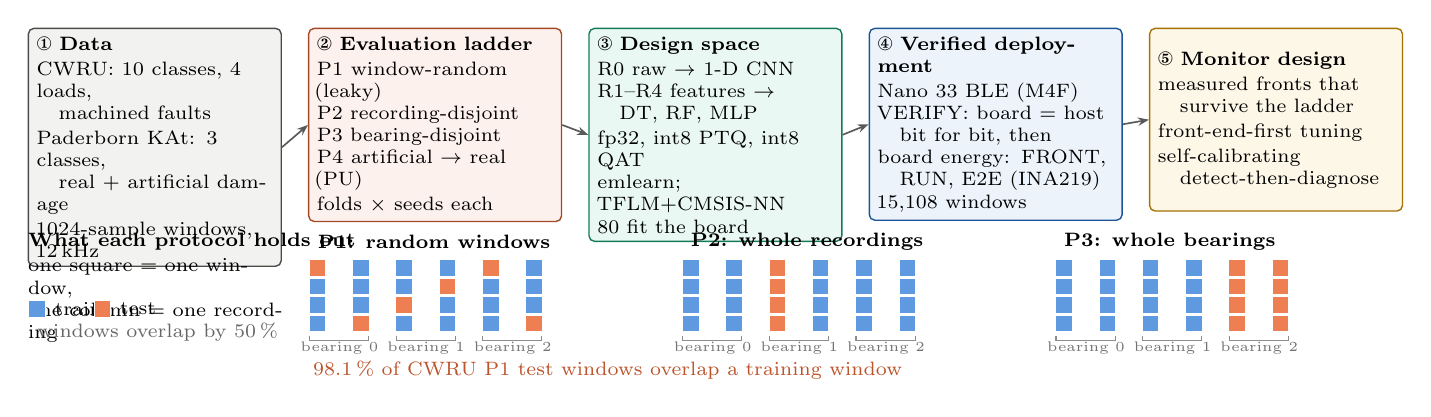
\begin{tikzpicture}[
  font=\scriptsize,
  >={Stealth[length=4pt]},
  blk/.style={draw=#1!70!black, fill=#1!9, rounded corners=2pt, line width=0.5pt, align=left,
              inner sep=3pt, text width=3.0cm, minimum height=2.32cm, anchor=north west},
  hd/.style={font=\scriptsize\bfseries, anchor=south west, inner sep=1pt},
  arr/.style={->, line width=0.6pt, draw=black!65},
  win/.style={minimum width=2.1mm, minimum height=2.1mm, inner sep=0pt, draw=white, line width=0.3pt},
]
\definecolor{cA}{HTML}{2A78D6}\definecolor{cB}{HTML}{EB6834}\definecolor{cC}{HTML}{1BAF7A}
\definecolor{cD}{HTML}{EDA100}\definecolor{cG}{HTML}{6B6B66}
\colorlet{tr}{cA!75}\colorlet{te}{cB!85}
% ---------------- top row: pipeline
\node[blk=cG] (d) at (0,0) {\textbf{\ding{172} Data}\\[1pt]
  CWRU: 10 classes, 4 loads,\\ \quad machined faults\\[1pt] Paderborn KAt: 3 classes,\\ \quad real + artificial damage\\[1pt]
  1024-sample windows, 12\,kHz};
\node[blk=cB] (p) at (3.56,0) {\textbf{\ding{173} Evaluation ladder}\\[1pt]
  P1 window-random (leaky)\\ P2 recording-disjoint\\ P3 bearing-disjoint\\ P4 artificial $\rightarrow$ real (PU)\\[1pt]
  folds $\times$ seeds each};
\node[blk=cC] (m) at (7.12,0) {\textbf{\ding{174} Design space}\\[1pt]
  R0 raw $\rightarrow$ 1-D CNN\\ R1--R4 features $\rightarrow$\\ \quad DT, RF, MLP\\[1pt]
  fp32, int8 PTQ, int8 QAT\\ emlearn; TFLM+CMSIS-NN\\ 80 fit the board};
\node[blk=cA] (b) at (10.68,0) {\textbf{\ding{175} Verified deployment}\\[1pt]
  Nano 33 BLE (M4F)\\ VERIFY: board = host\\ \quad bit for bit, then\\ board energy: FRONT,\\ \quad RUN, E2E (INA219)\\ \NumTotWindows{} windows};
\node[blk=cD] (o) at (14.24,0) {\textbf{\ding{176} Monitor design}\\[1pt]
  measured fronts that\\ \quad survive the ladder\\[1pt] front-end-first tuning\\[1pt]
  self-calibrating\\ \quad detect-then-diagnose};
\foreach \a/\b in {d/p,p/m,m/b,b/o} \draw[arr] (\a.east) -- (\b.west);
% ---------------- bottom row: what the protocols hold out (schematic)
\begin{scope}[yshift=-3.05cm]
  \node[anchor=west, font=\scriptsize\bfseries, inner sep=0pt] at (0,0.33) {What each protocol holds out};
  \node[anchor=north west, font=\scriptsize, text width=3.2cm, align=left, inner sep=0pt] at (0,0.12) {one square = one window,\\ one column = one recording};
  % legend
  \node[win, fill=tr] at (0.12,-0.52) {}; \node[anchor=west, font=\scriptsize] at (0.22,-0.52) {train};
  \node[win, fill=te] at (0.95,-0.52) {}; \node[anchor=west, font=\scriptsize] at (1.05,-0.52) {test};
  \node[anchor=west, font=\scriptsize, text=black!60] at (0,-0.82) {windows overlap by 50\,\%};
  % three protocol panels
  \foreach \px/\name/\mode in {3.56/P1: random windows/0, 8.3/P2: whole recordings/1, 13.04/P3: whole bearings/2}{
    \node[anchor=west, font=\scriptsize\bfseries] at (\px,0.33) {\name};
    \foreach \r in {0,...,5}{          % recordings (columns): bearings = pairs of recordings
      \foreach \w in {0,...,3}{        % windows in a recording
        \pgfmathtruncatemacro{\h}{mod(\r*7+\w*3,4)}
        \ifcase\mode
          \ifnum\h=0 \def\c{te}\else\def\c{tr}\fi
        \or
          \ifnum\r=2 \def\c{te}\else\def\c{tr}\fi
        \or
          \ifnum\r>3 \def\c{te}\else\def\c{tr}\fi
        \fi
        \node[win, fill=\c] at (\px+0.12+\r*0.55, 0.0-\w*0.235) {};
      }
    }
    % bearing brackets
    \foreach \bb in {0,1,2}{
      \draw[black!45, line width=0.4pt] (\px+0.02+\bb*1.1, -0.86) -- ++(0,-0.06) -- ++(0.75,0) -- ++(0,0.06);
      \node[font=\tiny, text=black!55] at (\px+0.4+\bb*1.1,-1.02) {bearing \bb};
    }
  }
  \node[anchor=west, font=\scriptsize, text=cB!80!black] at (3.5,-1.3)
       {\NumHostPOneLeakPct{} of CWRU P1 test windows overlap a training window};
\end{scope}
\end{tikzpicture}

\caption{Overview of \TJ{}. Top: the five stages from data to monitor design. Bottom: what each rung of the evaluation
ladder holds out (CWRU: P2 holds out a load, P3 a fault size, i.e.\ the physical bearing).}
\label{fig:overview}
\end{figure*}

Fig.~\ref{fig:overview} shows the five stages. Data enter an evaluation ladder (\ding{173}); every candidate in the
design space (\ding{174}) is deployed, verified and measured on the board (\ding{175}); and the monitor is designed
only from measured fronts that survive the ladder (\ding{176}).

\subsection{Evaluation ladder and robustness test}\label{sec:tj-ladder}
Each dataset is evaluated on protocols of increasing strictness: P1 splits windows at random (leaky); P2 holds out
whole recordings (a load or an operating condition); P3 holds out whole bearings; and, where the dataset allows, P4
trains on artificial and tests on real damage. Every protocol runs with five seeds, and P2--P4 test sets contain
non-overlapping windows only. A design conclusion is accepted only if it survives the ladder, which \TJ{} tests in
three ways: the Kendall rank correlation $\tau$ of models' macro-F1 between rungs, the survival of Pareto-optimal
models from P1 to P3, and the hypervolume \cite{zitzler1999multiobjective} of each model family on
$(1-\mathrm{F1},\ \log_{10}E,\ \log_{10}\mathrm{flash})$, min--max normalized per protocol with reference point 1.1.

\subsection{Design space}\label{sec:tj-space}
Five input representations cover the designs used in TinyML condition monitoring. R0 is the normalized raw window,
the CNN input. R1 holds ten time-domain statistics; R2 adds 14 log band energies of a Hann-windowed 1024-point FFT; R3
is a 256-bin log magnitude spectrum; and R4 is an envelope spectrum, i.e.\ R1 without its mean plus 32 log bins of the
demodulated 2--5\,kHz band, which carry the bearing defect frequencies \cite{randall2011rolling}. Removing the mean
from R4 is a leakage decision: the mean is the accelerometer's DC offset and fingerprints the recording
(\NumHostMeanZMax{}\,$\sigma$ outside the training range for one held-out file); with it, R4 MLPs reach macro-F1
\NumHostAblMeanWith{} on P2, without it \NumHostAblMeanWithout{}. The 88 model IDs comprise decision trees (depth 4--12)
and random forests (5--25 trees) on R1, R2 and R4, exported with emlearn \cite{nordby2019emlearn}; MLPs on R2--R4; and
1-D CNNs (four widths, two depths) on R0. All networks exist in fp32, post-training int8 and quantization-aware int8
and run under TFLM \cite{david2021tflm} with CMSIS-NN kernels \cite{lai2018cmsisnn}; \NumCwruNModels{} IDs fit the
board. Accuracy is the host macro-F1 averaged over folds and seeds; cost is measured on one deployed instance per ID,
since the operations do not depend on the weights except for tree path lengths (a whole forest inference costs at most
\NumPuRFRunMax\uJ{}).

\subsection{Verified deployment}\label{sec:tj-verify}
Host accuracy describes the board only if the board computes the same function. Before any energy window, \TJ{}'s
VERIFY gate sends 100 test vectors (10 per class) to the board and compares the outputs with the host reference: fp32
within $10^{-4}$, int8 within one quantization step and with identical classes, where the int8 reference is the
TFLite reference-kernel output that TFLM must reproduce bit for bit. Models that fail are not measured until fixed.
Energy is then measured in three modes, FRONT (front end only), RUN (classifier on stored features) and E2E (both),
each over $N$ calls in a window of at least 10\,s preceded by an IDLE window, and the dynamic energy per call is
\begin{equation}
E=\big(\bar P-\bar P_\mathrm{idle}\big)\,t/N ,
\label{eq:energy}
\end{equation}
with $t$ timed by the logger (Section~\ref{sec:setup-rig}).

\subsection{Self-calibrating detect-then-diagnose monitor}\label{sec:tj-mon}
Because a fault is rare, the monitor runs a cheap stage-1 gate on every window and wakes the stage-2 diagnosis model
only on an alarm. For fault prevalence $\pi$, the expected energy per window is
\begin{equation}
E(\pi)=E_1+\big[\pi\,\mathrm{TPR}+(1-\pi)\,\mathrm{FPR}\big]\,E_2 ,
\label{eq:cascade}
\end{equation}
so the gate pays off only if its false-alarm rate is low \emph{on the installed machine}. A factory-trained gate
fails this test whenever the operating point differs from training, and fault data from the installed machine never
exist. The \TJ{} gate therefore keeps one factory constant and learns the rest on the device from healthy vibration
(Algorithm~\ref{alg:cal}). It computes the R1 statistics in exact integer arithmetic on the raw int16 window, scores a
Mahalanobis distance to the healthy state, and, after installation, re-fits mean, covariance and threshold from the
first $n$ windows. Stage 2 reuses the gate's R1 features when its representation contains them.

\begin{algorithm}[t]
\caption{On-device calibration and monitoring}\label{alg:cal}
\begin{algorithmic}[1]
\Require factory ratio $\rho=\tau_\mathrm{f}/\mathrm{med}(d_\mathrm{val})$ of threshold to median healthy distance
\State \textbf{Calibrate} (once, at installation, no fault data):
\For{$i=1..n$ healthy windows $x_i$}
  \State $f_i\gets$ integer R1 features of $x_i$; Welford update of $\mu,\Sigma$
\EndFor
\State $\Sigma\gets\Sigma+10^{-3}I$; Cholesky factor of $\Sigma^{-1}$
\State $\tau\gets\rho\cdot\mathrm{median}_i\, d(f_i)$, \ $d(f)=\sqrt{(f-\mu)^\top\Sigma^{-1}(f-\mu)}$
\State \textbf{Monitor} (every window $x$):
\If{$d(f(x))>\tau$} run stage-2 diagnosis on $x$, reusing $f(x)$ \EndIf
\end{algorithmic}
\end{algorithm}

The monitor's hypotheses (board--host alarm agreement, measured gate cost, additivity of gate and model energy,
prediction of stream energy by Eq.~\eqref{eq:cascade}, calibration benefit and energy per hour), its gates, thresholds
and analysis were fixed in a protocol committed before the first cascade window \cite{nosek2018preregistration}.

% =====================================================================================================================
\section{Experimental Setup}\label{sec:setup}
\subsection{Datasets}
CWRU \cite{cwru,smith2015rolling} provides 40 drive-end recordings: normal and inner-race, ball and outer-race faults of
three sizes at four loads, i.e.\ ten classes, with one physical bearing per class. P2 holds out one load (four folds),
and P3 holds out one fault size (three folds, four classes), the only way to hold out a bearing on this dataset;
\NumHostPOneLeakPct{} of P1 test windows share samples with a training window. Paderborn KAt
\cite{lessmeier2016condition} provides 32 bearings (6 healthy, 12 with artificial and 14 with real damage) under four
operating conditions, used as three classes; P2 holds out a condition, P3 a quarter of the bearings of each class
(four folds), and P4 tests artificial-to-real transfer. Both datasets are resampled to 12\,kHz, low-pass filtered at
5\,kHz with one zero-phase FIR filter, and cut into 1024-sample windows (\NumWindowMs\,ms). The common filter matters:
without it, energy above 5.5\,kHz that is present only in CWRU fault files, an artefact of the recorder's anti-alias
roll-off, separates normal from faulty data on its own. Deployed instances are trained on CWRU P2 fold 0 and Paderborn
P3 fold 0.

\subsection{Measurement rig}\label{sec:setup-rig}
\begin{figure}[t]
\centering
\resizebox{\columnwidth}{!}{% Fig. 2 -- energy rig (a) and measurement window (b). Included from main.tex. Width = one column.
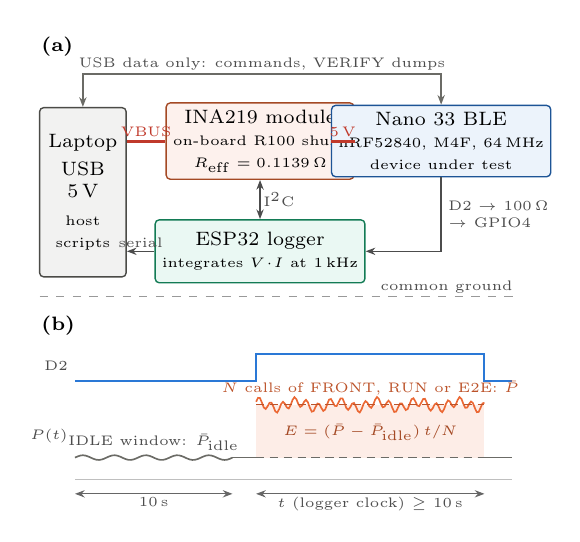
\begin{tikzpicture}[
  font=\scriptsize, >={Stealth[length=3.5pt]},
  box/.style={draw=#1!70!black, fill=#1!9, rounded corners=1.5pt, line width=0.5pt, align=center, inner sep=2.5pt},
  pw/.style={line width=1.1pt, draw=#1},
  sig/.style={->, line width=0.55pt, draw=black!70},
  lab/.style={font=\tiny, text=black!70, inner sep=1pt},
]
\definecolor{cA}{HTML}{2A78D6}\definecolor{cB}{HTML}{EB6834}\definecolor{cC}{HTML}{1BAF7A}
\definecolor{cD}{HTML}{EDA100}\definecolor{cG}{HTML}{6B6B66}\definecolor{vb}{HTML}{C0392B}
% ---------------- (a) wiring
\node[font=\scriptsize\bfseries, anchor=west] at (-0.15,2.75) {(a)};
\node[box=cG, minimum width=1.1cm, minimum height=2.15cm] (pc) at (0.5,0.9) {Laptop\\[2pt]USB\\5\,V\\[2pt]\tiny host\\\tiny scripts};
\node[box=cB, minimum width=1.7cm, minimum height=0.9cm] (ina) at (2.75,1.55) {INA219 module\\\tiny on-board R100 shunt\\\tiny $R_\mathrm{eff}=0.1139\,\Omega$};
\node[box=cA, minimum width=1.7cm, minimum height=0.9cm] (dut) at (5.05,1.55) {Nano 33 BLE\\\tiny nRF52840, M4F, 64\,MHz\\\tiny device under test};
\node[box=cC, minimum width=1.7cm, minimum height=0.8cm] (log) at (2.75,0.15) {ESP32 logger\\\tiny integrates $V\!\cdot\!I$ at 1\,kHz};
\draw[pw=vb] (pc.east|-ina.west) -- node[lab, above, text=vb]{VBUS} (ina.west);
\draw[pw=vb] (ina.east) -- node[lab, above, text=vb]{5\,V} (dut.west);
\draw[sig, <->, draw=cG] (pc.north) -- ++(0,0.42) -| node[lab, pos=0.25, above]{USB data only: commands, VERIFY dumps} (dut.north);
\draw[sig, <->] (ina.south) -- node[lab, right]{I$^2$C} (log.north);
\draw[sig] (dut.south) |- (log.east);
\node[lab, anchor=west, align=left] at (5.1,0.62) {D2 $\rightarrow$ 100\,$\Omega$\\$\rightarrow$ GPIO4};
\draw[sig] (log.west) -- node[lab, above]{serial} (pc.east|-log.west);
\draw[black!40, line width=0.4pt, dashed] (-0.05,-0.42) -- (6.0,-0.42);
\node[lab, anchor=east] at (6.0,-0.3) {common ground};
% ---------------- (b) one measurement block
\begin{scope}[yshift=-2.75cm]
\node[font=\scriptsize\bfseries, anchor=west] at (-0.15,1.95) {(b)};
\def\tA{0.4}\def\tB{2.4}\def\tC{2.7}\def\tD{5.6}
% D2 trace
\node[lab, anchor=east] at (0.35,1.45) {D2};
\draw[line width=0.7pt, cA] (0.4,1.25) -- (\tC,1.25) -- (\tC,1.6) -- (\tD,1.6) -- (\tD,1.25) -- (5.95,1.25);
% power trace
\fill[cB!12] (\tC,0.28) rectangle (\tD,0.95);
\node[lab, anchor=east, align=right] at (0.35,0.55) {$P(t)$};
\draw[black!25, line width=0.3pt] (0.4,0) -- (5.95,0);
\draw[line width=0.6pt, cG, domain=0.4:\tB, samples=60, smooth, variable=\x] plot (\x, {0.28+0.03*sin(900*\x)});
\draw[line width=0.6pt, cG] (\tB,0.28) -- (\tC,0.28);
\draw[line width=0.6pt, cB, domain=\tC:\tD, samples=120, variable=\x] plot (\x, {0.95+0.06*sin(2400*\x)+0.04*sin(700*\x)});
\draw[line width=0.6pt, cG] (\tD,0.28) -- (5.95,0.28);
\draw[densely dashed, cG, line width=0.4pt] (\tC,0.28) -- (\tD,0.28);
\draw[densely dashed, cB!80!black, line width=0.4pt] (\tC,0.95) -- (\tD,0.95);
\node[lab, anchor=south] at (1.4,0.33) {IDLE window: $\bar P_\mathrm{idle}$};
\node[lab, anchor=south, text=cB!80!black] at (4.15,1.03) {$N$ calls of FRONT, RUN or E2E: $\bar P$};
\draw[<->, line width=0.4pt, black!60] (\tC,-0.18) -- node[lab, below]{$t$ (logger clock) $\geq$ 10\,s} (\tD,-0.18);
\draw[<->, line width=0.4pt, black!60] (0.4,-0.18) -- node[lab, below]{10\,s} (\tB,-0.18);
\draw[densely dashed, cG, line width=0.4pt] (\tC,0.28) -- (\tD,0.28);
\node[font=\tiny, cB!70!black] at (4.15,0.6) {$E=(\bar P-\bar P_\mathrm{idle})\,t/N$};
\end{scope}
\end{tikzpicture}
}
\caption{(a) \TJ{} energy rig: the Nano's USB VBUS passes the INA219 shunt; the ESP32 logger integrates power over
windows framed by the Nano's D2 pin. (b) One measurement block: an IDLE window, then $N$ calls in a window of at
least 10\,s.}
\label{fig:rig}
\end{figure}

Fig.~\ref{fig:rig}(a) shows the rig. The Nano 33 BLE (nRF52840, Cortex-M4F at 64\,MHz) is powered from a laptop
through a cut USB cable whose VBUS line passes an INA219 module, while the data lines carry commands and VERIFY dumps.
An ESP32 logger reads bus voltage and shunt current at about 1\,kHz over I$^2$C and integrates power. The Nano's D2
pin, through 100\,$\Omega$ into an ESP32 input with a 100\,k$\Omega$ pull-down and a 100\,ms glitch filter, frames
each window, so both devices time the same interval. The module's R100 shunt was calibrated against 1\,k$\Omega$ and
100\,$\Omega$ $\pm$1\,\% resistors to an effective \NumRigShuntOhm\,$\Omega$; the residual $\pm$\NumRigShuntUnc\,\%
uncertainty scales all energies equally and leaves every comparison unchanged. The board runs from its crystal
oscillator, because the default RC oscillator ran \NumRigRcClockErr\,\% fast. Because $E$ in Eq.~\eqref{eq:energy} is
measured at the USB input, it includes the regulator and clock tree, i.e.\ the energy a board-level designer pays.

\subsection{Protocol and repeatability}
A window is rejected if the logger and board durations differ by more than 0.1\,\%, the INA219 overflows, the record
is incomplete or $t<10$\,s, and it is repeated up to three times; five stored inputs are measured per mode, and the
campaign is repeated three times on different days. It recorded \NumTotWindows{} windows in \NumTotSessions{}
sessions; \NumTotRejected{} were rejected (\NumCwruRejPct{} on CWRU, \NumPuRejPct{} on Paderborn) and re-measured.
Idle power was \NumCwruIdleMed\mW{} (5th--95th percentile \NumCwruIdleLo--\NumCwruIdleHi\mW{}). The median
repeat-to-repeat coefficient of variation of E2E energy is \NumCwruCvMed{} on CWRU and \NumPuCvMed{} on Paderborn
(worst \NumCwruCvMax{}), so differences above about 1\,\% are real, and E2E equals FRONT\,+\,RUN within a median
\NumCwruAddMed{}. Int8 models are reported from the patched library (Section~\ref{sec:res-pit}), so every energy
belongs to firmware whose outputs passed VERIFY. Table~\ref{tab:dec} lists the decisions behind these numbers.

\begin{table}[t]
\caption{Design decisions in TrueJoule and their rationale.}
\label{tab:dec}
\centering\footnotesize
\setlength{\tabcolsep}{3pt}
\begin{tabular}{@{}>{\raggedright\arraybackslash}p{3.05cm} >{\raggedright\arraybackslash}p{4.6cm}@{}}
\toprule
Decision & Reason \\
\midrule
\multicolumn{2}{@{}l}{\textit{Data and evaluation}}\\
Same 5\,kHz low-pass on all files & recorder roll-off otherwise labels CWRU faults \\
Non-overlapping P2--P4 test windows & no test sample seen in training \\
CWRU P3 = leave one fault size out & only way to hold out a bearing \\
Window mean dropped from R4 & DC offset fingerprints the recording \\
Host scoring with hard RF votes and TFLite reference int8 kernels & equals what emlearn and TFLM compute on the board \\
\multicolumn{2}{@{}l}{\textit{Measurement}}\\
Crystal clock (HFXO) & RC clock ran \NumRigRcClockErr\,\% fast \\
IDLE window before every block & tracks idle drift (\NumCwruIdleSpreadMW\,mW, 5--95\,\%) \\
Windows $\geq$\,10\,s, durations agree to 0.1\,\% & MLPerf Tiny rule; catches lost sync edges \\
Last accepted row per window & re-measured windows replace rejected ones \\
int8 energy from the patched library & every reported cost belongs to verified outputs \\
Both \texttt{log10f} builds reported & the fix changes R3 cost, not accuracy \\
\multicolumn{2}{@{}l}{\textit{Cascade}}\\
Protocol committed before the pilot & tests cannot be tuned to the outcome \\
Failed tests kept primary; G6 labelled post hoc & separates confirmation from exploration \\
\bottomrule
\end{tabular}
\end{table}

% =====================================================================================================================
\section{Results and Discussion}\label{sec:results}
\subsection{Which models survive the evaluation ladder}\label{sec:res-front}
\begin{figure*}[t]
\centering
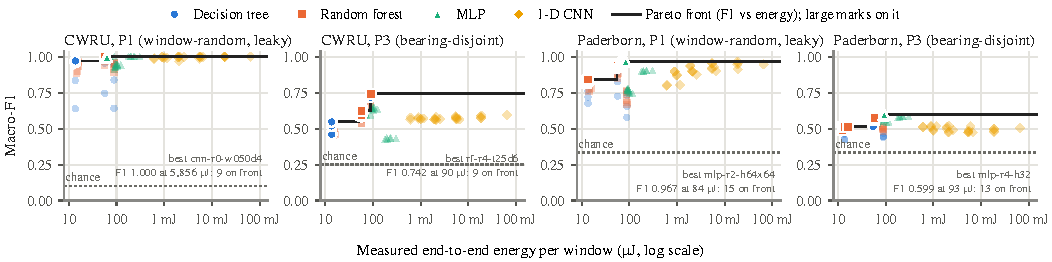
\includegraphics[width=\textwidth]{figs/fig_pareto.pdf}
\caption{Macro-F1 against measured end-to-end energy for the \NumCwruNModels{} deployed models on the leaky rung (P1)
and the bearing-disjoint rung (P3) of the ladder. Large markers and the step line form the Pareto front; faint markers
are dominated models. No CNN is Pareto-optimal on any rung.}
\label{fig:pareto}
\end{figure*}

Fig.~\ref{fig:pareto} shows the measured frontiers. On P1 the most accurate CWRU model is a CNN
(\NumCwruPOneBestId{}, F1 \NumCwruPOneBest{} at \NumCwruPOneBestE\uJ{}), yet a forest (\NumCwruPOneNearId{}) is within
0.01 F1 for \NumCwruPOneNearSaving$\times$ less energy. On P3 the best model is \NumCwruPThreeBestId{} (F1
\NumCwruPThreeBest{} at \NumCwruPThreeBestE\uJ{}), against \NumCwruPThreeBestCNN{} for the best CNN and
\NumCwruPThreeBestMLP{} for the best MLP. The ladder is not a uniform discount: only \NumCwruFrontKept{} of the
\NumCwruFrontPOneN{} models on the CWRU P1 front remain on the P3 front (\NumPuFrontKept{} of \NumPuFrontPOneN{} on
Paderborn), and Kendall $\tau$ between the P1 and P3 rankings is \NumCwruTauPOnePThree{} on CWRU and
\NumPuTauPOnePThree{} on Paderborn (\NumPuTauPOnePFour{} between P1 and P4). The median macro-F1 loss from P1 to P3 is
\NumCwruDropAll{} on CWRU, smallest for trees (\NumCwruDropDT{}) and largest for CNNs (\NumCwruDropCNN{}).

With flash as the third objective, the family hypervolume ranking on CWRU stays \NumCwruRankPOne{} along the ladder,
because trees dominate the memory axis, whereas on Paderborn it moves from \NumPuRankPOne{} on P1 to \NumPuRankPLast{}
on P3, where the envelope-feature MLP \NumPuPThreeBestId{} (F1 \NumPuPThreeBest) leads. Rankings also do not carry
across datasets: $\tau$ between the CWRU and Paderborn P3 rankings is \NumTauCwruPuPThree{}, and the best CWRU P3 model
ranks \NumCwruBestRankOnPu{} of \NumNModelsBoth{} on Paderborn. A monitor must therefore be selected on the strictest
rung of its own machine's data, and selecting it on P1 would have shipped a CNN that costs
\NumCwruCnnOverTreeMin--\NumCwruCnnOverTreeMax$\times$ the cheapest tree.

\subsection{Where the energy of a decision goes}\label{sec:res-energy}
\begin{table}[t]
\caption{Measured cost and host accuracy per family (CWRU energy and memory; Paderborn energies agree within a few
per cent). F1: best macro-F1 under P1 / P3.}
\label{tab:fam}
\centering\footnotesize
\setlength{\tabcolsep}{2.6pt}
\begin{tabular}{@{}l c c c c c c@{}}
\toprule
 & $n$ & E2E (\textmu J) & Latency (ms) & Flash (KB) & F1 CWRU & F1 PU \\
\midrule
DT  & \NumCwruDTN & \NumCwruDTEMin--\NumCwruDTEMax & \NumCwruDTTMinMs--\NumCwruDTTMaxMs & \NumCwruDTFlashMinKB--\NumCwruDTFlashMaxKB & \NumCwruPOneBestDT\,/\,\NumCwruPThreeBestDT & \NumPuPOneBestDT\,/\,\NumPuPThreeBestDT \\
RF  & \NumCwruRFN & \NumCwruRFEMin--\NumCwruRFEMax & \NumCwruRFTMinMs--\NumCwruRFTMaxMs & \NumCwruRFFlashMinKB--\NumCwruRFFlashMaxKB & \NumCwruPOneBestRF\,/\,\NumCwruPThreeBestRF & \NumPuPOneBestRF\,/\,\NumPuPThreeBestRF \\
MLP & \NumCwruMLPN & \NumCwruMLPEMin--\NumCwruMLPEMax & \NumCwruMLPTMinMs--\NumCwruMLPTMaxMs & \NumCwruMLPFlashMinKB--\NumCwruMLPFlashMaxKB & \NumCwruPOneBestMLP\,/\,\NumCwruPThreeBestMLP & \NumPuPOneBestMLP\,/\,\NumPuPThreeBestMLP \\
CNN & \NumCwruCNNN & \NumCwruCNNEMin--\NumCwruCNNEMax & \NumCwruCNNTMinMs--\NumCwruCNNTMaxMs & \NumCwruCNNFlashMinKB--\NumCwruCNNFlashMaxKB & \NumCwruPOneBestCNN\,/\,\NumCwruPThreeBestCNN & \NumPuPOneBestCNN\,/\,\NumPuPThreeBestCNN \\
\bottomrule
\end{tabular}
\end{table}

\begin{figure}[t]
\centering
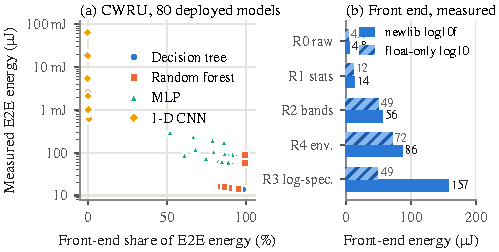
\includegraphics[width=\columnwidth]{figs/fig_energy.pdf}
\caption{(a) Front-end share of measured E2E energy against E2E energy (CWRU). (b) Measured front-end energy per
representation with the newlib \texttt{log10f} and with a float-only logarithm; R0/R1 contain no logarithm, so
their change shows the effect of the firmware image alone.}
\label{fig:energy}
\end{figure}

Fig.~\ref{fig:energy}(a) and Table~\ref{tab:fam} split each decision into its two halves. For trees and forests the
classifier is almost free: a tree inference costs \NumCwruDTRunMin--\NumCwruDTRunMax\uJ{} and a forest
\NumCwruRFRunMin--\NumCwruRFRunMax\uJ{}, so the front end accounts for \NumCwruDTFrontShare{} and
\NumCwruRFFrontShare{} of their E2E energy, and the representation alone sets the energy tier: R1
\NumCwruFrontROne\uJ{}, R2 \NumCwruFrontRTwo\uJ{}, R4 \NumCwruFrontRFour\uJ{}, R3 \NumCwruFrontRThree\uJ{}. MLPs spend
\NumCwruMLPFrontShare{} of their energy in the front end, whereas CNNs (\NumCwruCnnEMinMJ--\NumCwruCnnEMaxMJ\,mJ) spend
almost all of it in inference. Both datasets agree within a few per cent (Paderborn: R1 \NumPuFrontROne\uJ{}, R4
\NumPuFrontRFour\uJ{}). The lever for a feature-based monitor is therefore its front end.

Pulling that lever paid off at once. The R3 cost stood out in the comparison with estimates
(Section~\ref{sec:res-est}) and traced to the GCC~7 newlib \texttt{log10f}, which computes in double precision on a
single-precision FPU. A float-only logarithm (\NumRigFloatLogCycles{} instead of \NumRigLogfCycles{} cycles, error
below $\NumRigFloatLogErr$) cuts the R3 front end from \NumCwruFrontRThree{} to \NumCwruLfFrontRThree\uJ{}
(\NumCwruLfFactorRThree$\times$; Paderborn \NumPuLfFactorRThree$\times$) and the E2E energy of R3 MLPs by up to
\NumCwruLfEtoeSaveMax{}. R2 and R4, which take 14 and 32 logarithms, become \NumCwruLfSaveRTwo{} and
\NumCwruLfSaveRFour{} cheaper. R1, which takes none, also moves (\NumCwruLfChangeROne{} on CWRU,
\NumPuLfChangeROne{} on Paderborn), and single R0 and R1 front ends move by up to \NumLfImageShiftMax\,\% in either
direction: rebuilding the firmware alone changes the time and power of unchanged code, as it already did between
bundles of the original campaign. \TJ{} therefore treats the firmware image as a systematic and reports both builds
(\NumCwruLfReps{} repeats per model on CWRU, \NumPuLfReps{} on Paderborn).

\subsection{Why the energy must be measured}\label{sec:res-est}
\begin{figure}[t]
\centering
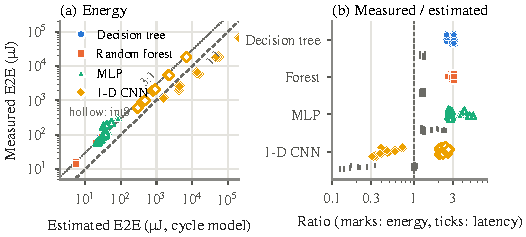
\includegraphics[width=\columnwidth]{figs/fig_est.pdf}
\caption{(a) Measured against chip-level estimated E2E energy (CWRU). (b) Measured/estimated ratio per family for
energy (markers; hollow: int8) and latency (ticks).}
\label{fig:est}
\end{figure}

Before the board was available, every model had been costed with an instruction-accurate emulator, a Cortex-M4 cycle
model and datasheet power, which is the usual practice. Fig.~\ref{fig:est} compares this estimate with the board. It
orders the models well (Spearman $\rho=\NumCwruEstSpearman$) but misses their energy by
\NumCwruEstRatioMin--\NumCwruEstRatioMax$\times$ (median \NumCwruEstRatioMed$\times$), and the error depends on the
model: trees and forests lie at \NumCwruEstRatioTreeMin--\NumCwruEstRatioTreeMax$\times$, int8 networks above that, and
fp32 CNNs below one, because the cycle model overestimates floating-point convolution. Latency ratios span
\NumCwruLatRatioMin--\NumCwruLatRatioMax; the largest CNN was predicted at \NumCwruBigCnnEstS\,s per inference and takes
\NumCwruBigCnnMeasS\,s. The error is large enough to move models on and off the front: with estimated energy,
\NumCwruPThreeEstFrontDiff{} models change Pareto status on the CWRU P3 front and \NumPuPThreeEstFrontDiff{} on the
Paderborn P3 front, and no single correction factor repairs this.

\subsection{What verification caught}\label{sec:res-pit}
\begin{table}[t]
\caption{Deployment pitfalls found by output verification or measurement.}
\label{tab:pit}
\centering\footnotesize
\setlength{\tabcolsep}{3pt}
\begin{tabular}{@{}>{\raggedright\arraybackslash}p{2.25cm} >{\raggedright\arraybackslash}p{3.45cm} >{\raggedright\arraybackslash}p{1.9cm}@{}}
\toprule
Pitfall & Effect & Found by \\
\midrule
Per-channel int8 dense layers ignored by Arduino TFLM port & wrong int8 outputs; class agreement down to
\NumPuVerIntAgreeMin{}; energy unchanged & VERIFY \\
int8 MEAN rounding & 1 LSB in \NumRigMeanLsbLo--\NumRigMeanLsbHi\,\% of pooled values & layer-wise VERIFY \\
newlib \texttt{log10f} in double precision & R3 front end \NumCwruLfFactorRThree$\times$ too costly & estimate audit \\
Firmware image layout & same front end up to $\pm$\NumLfImageShiftMax\,\% & repeated builds \\
RF soft vs.\ hard voting & host and board predictions differ & emulator VERIFY \\
\bottomrule
\end{tabular}
\end{table}

Table~\ref{tab:pit} lists the faults that VERIFY and the measurements exposed. The most consequential is silent. On
the unpatched Arduino TFLM library, VERIFY passed all fp32 networks and trees but failed \NumCwruVerIntFail{} of
\NumCwruVerIntN{} int8 models on CWRU and \NumPuVerIntFail{} of \NumPuVerIntN{} on Paderborn, with class agreement as
low as \NumPuVerIntAgreeMin{}. The port applies a single requantization multiplier to fully-connected layers whose
weights TF\,2.18 quantizes per channel, and the int8 MEAN (global average pooling) rounds differently from the
reference. The energy campaign could not have noticed: patched and unpatched int8 E2E energies differ by a factor of
\NumCwruPatchRatioMin--\NumCwruPatchRatioMax{} (median \NumCwruPatchRatioMed), because the fault changes arithmetic,
not work. After a two-file patch, \NumCwruVerTwoPass{} of \NumCwruVerTwoN{} TFLM models pass on both datasets with
bit-exact int8 outputs. Without the VERIFY gate, a measurement study would have reported correct costs for incorrect
models. The forest voting mismatch (scikit-learn averages probabilities, emlearn takes a majority vote) is resolved by
scoring forests with hard voting on the host.

\subsection{The self-calibrating monitor on the board}\label{sec:res-cas}
\begin{figure}[t]
\centering
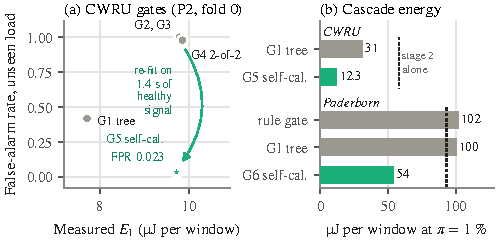
\includegraphics[width=\columnwidth]{figs/fig_cascade.pdf}
\caption{(a) Measured stage-1 energy and false-alarm rate at the unseen load for the CWRU gates; the factory
healthy-only gate alarms on every healthy window until it re-fits itself on the device. (b) Energy per window at 1\,\%
fault prevalence; dashed: stage-2 model alone.}
\label{fig:cascade}
\end{figure}

We compared the self-calibrating gate (G5) with a depth-limited tree gate (G1), factory healthy-only Mahalanobis gates
(G2, G3) and a two-in-a-row confirmation (G4), all on integer R1 features, over three repeats per dataset. All
\NumCwruCasChecks{} (CWRU) and \NumPuCasChecks{} (Paderborn) board alarms agreed with the host, including after on-device
calibration. A gate decision costs \NumCwruGateEMin--\NumCwruGateEMax\uJ{} per window,
\NumCwruGateRatioMin--\NumCwruGateRatioMax$\times$ the chip-level estimate. Fig.~\ref{fig:cascade}(a) shows why the
gate must calibrate itself: at the unseen load of the deployed CWRU split, the factory healthy-only gates alarm on
every healthy window (FPR \NumCasCwGTwoFpr{}) and the tree gate on \NumCasCwGOneFpr{} of them. After re-fitting on
\NumCasCalibSixteenS\,s of healthy vibration, G5 reaches FPR \NumCasCwGFivenOneSixFpr{} at TPR
\NumCasCwGFivenOneSixTpr{} (across all P2 folds, \NumCasCwFactoryFprAll{} $\rightarrow$ \NumCasCwSelfFprAll{}). At
$\pi=1\,\%$, the monitor spends \NumCasEpiCwruGFive\uJ{} per window against \NumCwruPTwoBestE\uJ{} for the diagnosis
model alone, a \NumCasCwSaving$\times$ reduction; the one-time calibration costs \NumCwruCalibGFiveNOneSix\uJ{} and is
repaid after about \NumCasCwPayback{} windows.

On Paderborn the pre-registered gate selection failed: every candidate with TPR\,$\geq$\,0.98 had FPR 1.0
(\NumCasPuRuleNPass{} of \NumCasPuRuleNGates{}), so the selected gate escalates every window and the cascade costs
\NumCasPuRuleE\uJ{} against \NumCasPuModelE\uJ{} for the model alone. Extending self-calibration to R1 plus band
features (G6, chosen after the study and reported as such) gives FPR \NumCasPuSixNOneTwoEightFprPThree{} on P3 and
\NumCasPuSixNOneTwoEightFprPFour{} on the held-out P4, for \NumCasEpiPuGSix\uJ{} per window
(\NumCasPuSaving$\times$). Self-calibration is thus what makes the gate useful on both machines. Two pre-registered
prediction tests failed and stay reported: additivity of gate and model energy against the main campaign ($\Delta$
down to \NumCwruRqThreeMin{} on CWRU and \NumPuRqThreeMin{} on Paderborn) and stream-energy prediction within 3\,\%
(\NumCwruRqFourFail{} of \NumCwruRqFourN{} CWRU and \NumPuRqFourFail{} of \NumPuRqFourN{} Paderborn streams). The
additivity failures and the CWRU stream failures trace to the firmware-image systematic of
Section~\ref{sec:res-energy}: within one image, additivity holds to \NumCwruRqThreeInMin--\NumCwruRqThreeInMax{} and
CWRU streams to within \NumCwruRqFourInMax{}, whereas Paderborn streams still exceed the prediction by
\NumPuRqFourInMin--\NumPuRqFourInMax{}, an overhead we attribute, untested, to reading stream windows from flash.
Duty-cycled at one window per second, monitoring adds \NumCwruIncJhOneS\,J/h (CWRU) and \NumPuIncJhOneS\,J/h
(Paderborn) to a board that idles at about \NumCwruIdleJh\,J/h, so with \TJ{}'s monitor the node's lifetime is set by
its sleep power, not by diagnosis.

\subsection{Design guidelines}\label{sec:guide}
The measurements condense into five guidelines for vibration TinyML monitors. (i) Select on the strictest rung of the
ladder for the target dataset; on unseen bearings, a forest on R2/R4 features (CWRU, \NumCwruPThreeBestE\uJ{} per
decision) or an envelope-feature MLP (Paderborn, \NumPuPThreeBestE\uJ{}) dominates. (ii) Optimize the front end before
the classifier: it holds most of the energy, and one C-library call changed it threefold. (iii) Verify outputs on the
board before measuring, especially for int8 models. (iv) Treat estimates as rankings, not budgets, and the firmware
image as a systematic. (v) Calibrate the wake-up gate on the installed machine; a factory gate can cost more than no
gate at all.

\textbf{Limitations.} Energies are board-level at the 5\,V USB input of one board; core-rail energies are lower. The
shunt was calibrated without a DMM. CWRU has one bearing per class, so its P3 normal class is split by load, and CWRU
gate choices used test-split host scores, so detection claims rest on Paderborn's held-out P4. Costs come from one
deployed instance per architecture, fp32 CNN energies of the first three repeats carry a $\pm$2\,\% library-layout
systematic, and G6 was chosen after the study.

% =====================================================================================================================
\section{Conclusion and Future Work}\label{sec:concl}
This paper introduced \TJ{}, a framework that admits a number into a TinyML design decision only after it has been
measured on the board, produced by verified outputs and confirmed on unseen bearings, and used it to build a
self-calibrating detect-then-diagnose bearing monitor on a Cortex-M4F. Applied to \NumCwruNModels{} models and two
datasets, the framework changed the design at every step. Bearing-disjoint evaluation replaced the CNN that the leaky
protocol favoured with a forest or an envelope-feature MLP at a fraction of its energy; measured front-end energy
redirected optimization from the classifier to the feature extractor, where a single library fix saved a factor of
\NumCwruLfFactorRThree; board verification removed an int8 fault that measurement alone would have hidden; and a
gate that calibrates itself from \NumCasCalibSixteenS\,s of healthy vibration lowered false alarms at an unseen load
to \NumCasCwGFivenOneSixFpr{} and the monitor's energy \NumCasCwSaving$\times$. The result is a monitor whose accuracy,
energy and behaviour after installation can be predicted before it is mounted, which is what a maintenance engineer
needs from a sensor that will run unattended for years.

Future work will extend \TJ{} to core-rail measurement and to MCUs without an FPU, where integer and fixed-point front
ends change the energy ranking; run the self-calibrating monitor on battery-powered nodes on operating machines; and
release the rig design, firmware and all \NumTotWindows{} measurement windows so that other TinyML studies can be
checked against the same procedure.

\section*{Acknowledgment}
The authors used Claude (Anthropic) to assist with the literature analysis, analysis scripts, figures and drafting;
all measurements, results and conclusions were produced and checked by the authors.

\bibliographystyle{IEEEtran}
\bibliography{references}

\end{document}
